\documentclass[review]{elsarticle}
%%\usepackage[utf8]{inputenc}
%%\usepackage[LGR,T1]{fontenc}
%%\usepackage{graphicx,amsmath}
%%\usepackage[british]{babel}
%%\usepackage[latin9]{inputenc}%SOME KIND OF CLASH WITH THIS ONE
%%\usepackage{array}
%%\usepackage{rotfloat}
%%\usepackage{textcomp}
%%\usepackage{amssymb}
\usepackage{amsmath} 
%% to align equations \usepackage{mathrsfs} % curly font in math, called using mathscr
%%\usepackage{graphicx}
%%\usepackage{subcaption} % to have two images under one caption
%%\usepackage{subscript}
%%\usepackage{gensymb} %for degree symbol
\setlength{\marginparwidth}{4cm} % to set the width of the marginpar
\usepackage{todonotes}
%%\usepackage{xargs}                      % Use more than one optional parameter in a new commands
%%\renewcommand{\baselinestretch}{1.5}
\bibliographystyle{elsarticle-num}
\begin{document}
\begin{frontmatter}
\title{Advanced novel characterisation of nuclear graphite microstructure via inverse modelling of Scanning Electron Microscopy, N$_2$ adsorption and Hg porosimetry}
\author[plym]{Bradley Moresby-White}
\author[plym]{Katie L. Jones\corref{cor1}}
\ead{katie.jones@plymouth.ac.uk}
\author[plym]{G. Peter Matthews}
\author[plym]{Giuliano M. Laudone}
\cortext[cor1]{Corresponding author.}
\address[plym]{Faculty of Science and Engineering, University of Plymouth, Plymouth, UK}
\begin{abstract}
Nuclear grade graphite
\end{abstract}
\begin{keyword}keyword\sep keyword\sep keyword\end{keyword}
\end{frontmatter}
\section{Introduction}
\section{Methodology}

\subsection{Materials}
\todo{NUMBER, SPACE, UNIT}

Virgin graphite samples of two grades, IG-110 and IG-430, were supplied by Toyo
Tanso Ltd\texttrademark{}, Osaka, Japan. The properties of both grades are
tabulated (Table ~\ref{tab:materialstable}). IG‑110 is employed in the
three existing HTGRs worldwide, while IG‑430 is designed to deliver increased
density, strength, and thermal conductivity for future
applications.\citep{toyotanso_atomic_nuclear} (Table ~\ref{tab:materialstable}).

\todo{for the following table,, check the big american review paper also and cite it.}
\todo{careful not too many self citations}
\begin{table*}
  \centering
  \caption{Manufacturer dataset for IG-110 and IG-430 \citep{Jones2018, ARREGUIMENA2022112047}}
  \label{tab:materialstable}
  \resizebox{\textwidth}{!}{%
    \begin{tabular}{l l c c c c c}
      \hline
      Grade   & Coke source & Bulk density/g cm$^3$ & Filler particle size/$\mu$m) & Tensile strength/MPa & Young's modulus/GPa & Thermal conductivity/W m$^{-1}$K$^{-1}$\\
      \hline
      IG‑110  & Petrol          & 1.77                  & 10                           & 25                     & 9.8                   & 120 \\
      IG‑430  & Pitch             & 1.82                  & 10                           & 37                     & 10.8                  & 140 \\
      \hline
    \end{tabular}%
  }
\end{table*}

\subsection{Sample preparation}
Cuboids were subsampled from virgin graphite blocks, with dimensions of
approximately 10 mm x 10 mm x 100 mm. The subsamples were further subsampled into
cuboids of side lengths ~ 7 mm, providing 3 cuboids per grade. Samples were
polished via SiC polishing pads up to a grit size of P5000, to minimise
topographical variations induced by sample preparation that may cause artefacts
during SEM imaging or low pressure gas adsorption \citep{Fang2022,Jones2018}.
Samples were sonicated in 2-propanol for 24 h to remove any contaminants, such as
silica particles introduced during polishing, then dried under vacuum
for 12 h at $305 \pm 5 \,^\circ\mathrm{C}$ using the BELPREP-vac (MicrotracBEL,
Japan) to remove any residual moisture introduced during sonication.

\todo{Could talk here about how we wanted to do resin impeg like Kane et al, but
  did not have the chance, and explain this might introduce issues, also we
  could talk about how this is quite rough, and that this kind of sample
  preparation (i.e. no vibratory polishing, no resin impregnation) is not ideal
  and may have introduced both artefacts and noise. Additionally, sonication may
  have damaged the pore structure}

\subsection{Scanning Electron Microscopy (SEM)}

The JEOL IT510 Scanning Electron Microscope was employed to generate the
contiguous set of individual micrographs from which the full composite
micrograph was assembled. The Image Montage capability within the JEOLInScope
package performed this function, capturing multiple micrographs via a motorized
stage, moving the electron beam over the specified area with a set overlap for
each new micrograph. Stigmation, contrast, and brightness are automatically
adjusted, with analysis of the metadata for all 1,350 micrographs demonstrating
that shifts in contrast and brightness were insignificant, with no impact on the
selection of the intensity threshold for the full composite (Table
~\ref{tab:contrast-brightness-summary}). Applied parameters are tabulated (
Table ~\ref{tab:microscopy_parameters}).

\begin{table}[ht]
  \centering
  \caption{Contrast (C) and Brightness (C) Summary by Sammple}
  \label{tab:contrast-brightness-summary}
  \resizebox{\columnwidth}{!}{%
  \begin{tabular}{lrrrr}
    \hline
    Variant & Avg C (\%) & Std C (\%) & Avg B (\%) & Std B (\%) \\
    \hline
    IG430B & 98.01 & 1.02 & 99.69 & 0.08 \\
    IG430C & 98.16 & 0.82 & 99.83 & 0.08 \\
    IG110B & 95.86 & 0.72 & 99.26 & 0.13 \\
    IG110C & 94.03 & 0.93 & 99.38 & 0.13 \\
    IG110F & 98.20 & 0.70 & 99.69 & 0.13 \\
    \hline
  \end{tabular}
  }
\end{table}

\begin{table}
  \centering
  \caption{Parameters for composite assembly captured with the JEOL IT510 SEM using Image Montage Mode}
  \label{tab:microscopy_parameters}
  \begin{tabular}{l l}
    \hline
    Parameters & Values \\
    \hline
    Magnification ($\times$)                    & 1000 \\
    Resolution ($\mu$m/px)               & 0.1 \\
    Surface area per micrograph ($\mu$m$^2$) & 12\,288 \\
    Overlap (\%)                          & 10 \\
    Micrographs per sample (n)            & 196 \\
    \hline
  \end{tabular}%
\end{table}

A magnification of 1000X was selected as a compromise between a resolution
sufficient for capturing the pore structure and area covered by each micrograph.
Each micrograph represents 12,288 µm² of sample surface, with each sample
consisting of 225 micrographs, yielding a total imaging area of 2.765 mm² per
sample. With 3 samples analysed per grade, the total scanned area per graphite
grade is 8.294 mm². 
\todo{Huang 2021 used 5000× magnification with 48 micrographs per sample, covering 0.13 mm × 0.13 mm for their composite.}
\todo{I actually did 0-14 so that is 15 x 15 which is 225 micrographs per sample, not 196.}

\subsection{Composite assembly}
\todo{5625}
Stitching/composite assembly, where the overlapping micrographs are assembled
into a single composite per sample, was performed via an enhanced phase
correlation type method, operated as an ImageJ plugin \citep{ Preibisch2009}.

This method optimises micrograph position globally, is sub-pixel accurate and
smooths the transitions between micrographs by a non-linear intensity blending
function. Further information on the exact function of this can be found in the
Supplementary Information.

The resulting composite micrographs display no visible delineation between
individual micrographs, cover an area comparable with previous works, are of
high resolution, and distinguish porosity and bulk (Figure \ref{fig:IG430C split
scaled} \citep{Huang2019,Kane2011a}). 

	\begin{figure}
		\centering
		\includegraphics[width=0.45\textwidth]{./Media/C1-IG430c fusion cropped split scaled.jpg}
		\caption{Fully assembled SEM composite: IG-430 Sample C, 1000×  magnification,
     5 kV accelerating voltage. Bar = 250 µm.}
		\label{fig:IG430C split scaled}
	\end{figure} 

	\subsection{Computation of Channel Porosity}
\subsubsection{Intensity/Greyscale Thresholding}

Per 8-bit micrograph \(E\) (pixel values \(0 \le E(x,y) \le 255\)), the
intensity histogram \(H(i)\) is computed for \(i=0,1,\dots,255\).
\[
H(i) = \sum_{x=1}^{M}\sum_{y=1}^{N} \mathbf{1}\{E(x,y)=i\},
\]
where \(M\) and \(N\) are the micrograph width and height (in pixels), and
\[
\mathbf{1}\{E(x,y)=i\} =
\begin{cases}
1, & \text{if the pixel at }(x,y)\text{ has intensity }i,\\
0, & \text{otherwise.}
\end{cases}
\]

The indicator function \(\mathbf{1}\{E(x,y)=i\}\) yields 1 where a given pixel
greyscale value equals \(i\), and 0 otherwise. The double sum
\(\sum_{x=1}^M\sum_{y=1}^N\) performs this operation across each pixel in the
micrograph resulting in a histogram \(H(i)\) of 256 bins, each bin representing
number of pixels in the micrograph at each greyscale value \(i\). 

Intensity thresholding, performed on \(H(i)\), determines a greyscale value
at which porosity and bulk (i.e., foreground and background) are distinguished.

Global automatic thresholding algorithms optimise by different criteria (i.e.
maximisation of inter-class variance, minimisation of intra-class variance) to
determine threshold(s). Thresholding aims to select an intensity value that classifies
porosity and bulk in a way that minimises both Type I and II errors, as
evaluated by the operator (i.e., false positives, classifying a pore where one
is not present, and false negatives, not classifying a pore where one is
present).

A test of all 17 of the available automatic thresholding methods available in
ImageJ demonstrated that none of the available automatic global intensity
thresholding algorithm effectively distinguished between porosity and bulk with
the sensitivity required to allow the classification of pores for the given
histogram (Figure ~\ref{fig:Try All Thresholding Methods}). This is primarily
because no histogram \(H(i)\) generated by this method exhibited more than one
peak, this statistically there were no classes to be separated (Figure
~\ref{fig:histogramnobimodal}). 

Evaluation of all 17 automatic global intensity thresholding algorithms
available in ImageJ revealed that non were able to distinguish between porosity
and bulk with the sensitivity required to allow the classification of pores for
the given histogram (Figure ~\ref{fig:Try All Thresholding Methods}). In every
case, the histogram \(H(i)\) produced by this method exhibited only a single
peak, yielding no statistically distinct intensity classes (Figure
\ref{fig:histogramnobimodal}). Automatic thresholding selects a threshold
between modes/classes, consequently, no global intensity thresholding method
could distinguish porosity and bulk in this dataset.

    \begin{figure}
		\centering
    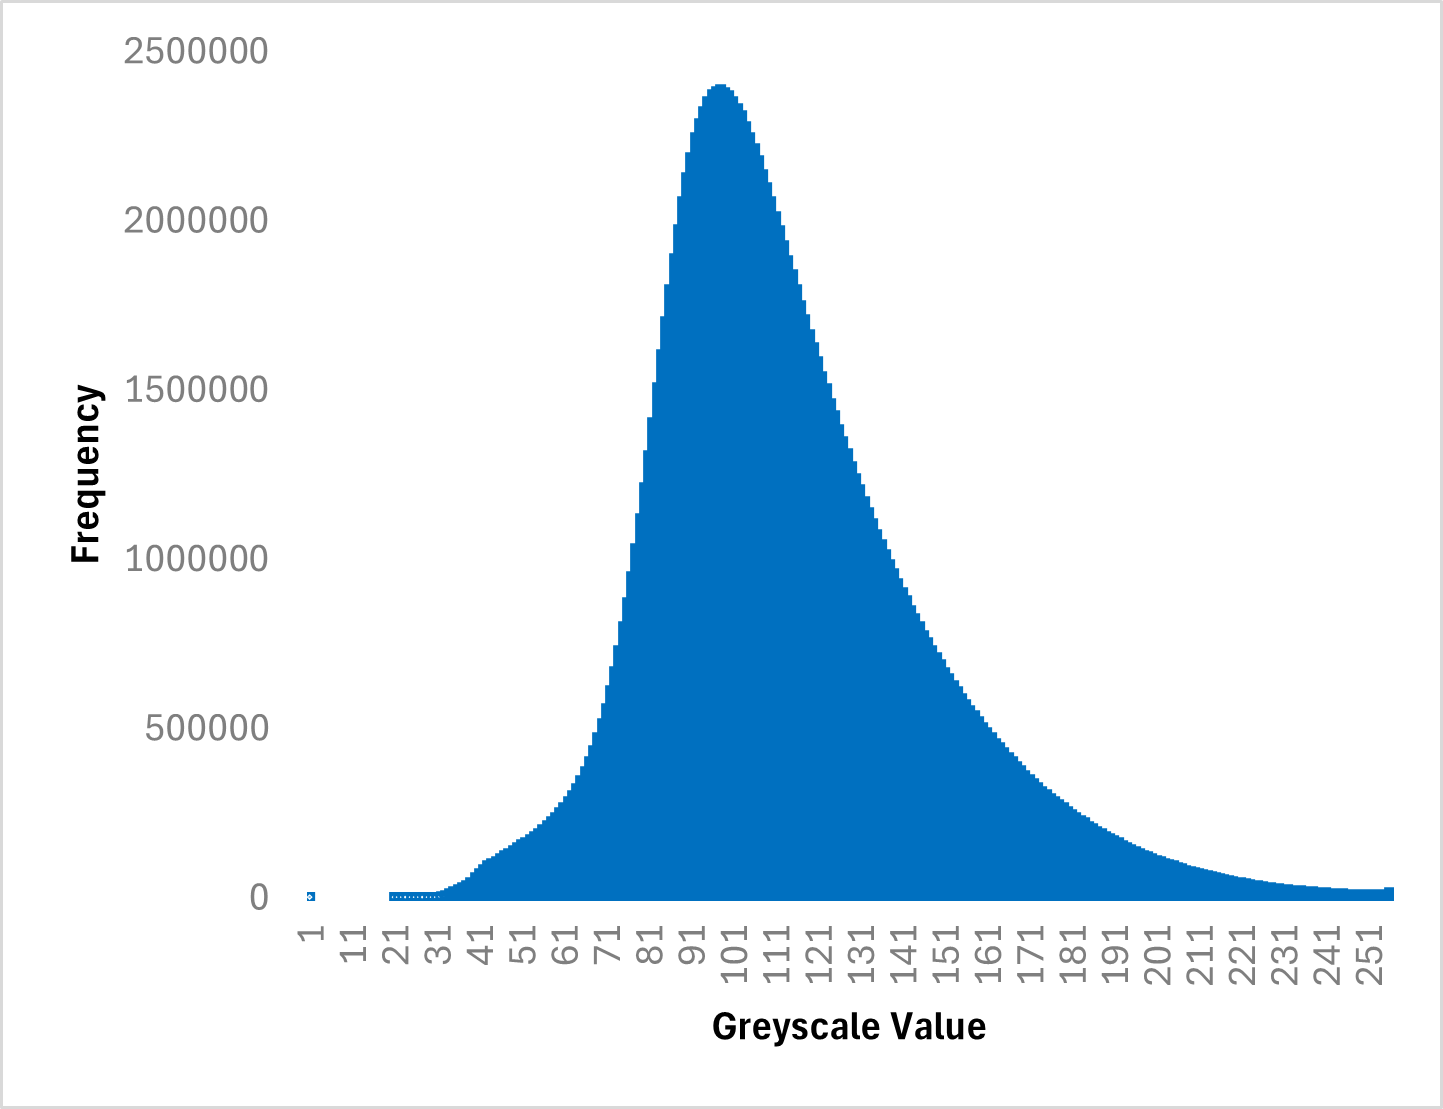
\includegraphics[width=0.45\textwidth]{./Media/IG430F Greyscale Histogram.png}
		\caption{PLACEHOLDER DRAFT: Histogram of greyscale values for IG-430 Sample F, 1000×, Showing skewness and unimodality}
		\label{fig:histogramnobimodal}
	\end{figure} 

	\begin{figure}[!htbp]
		\centering
		\includegraphics[width=0.45\textwidth]{./Media/MontageIG430C Methods.jpg}
		\caption{Thresholded Micrograph of IG-430 Sample C at $1000\times$ Magnification. Methods are placed sequentially from right to left, row by row. 
      (a) Default
			(b) Huang
			(c) Huang2
			(d) Intermodes
			(e) IsoData
			(f) Li
			(g) MaxEntropy
			(h) Mean
			(i) MinError(I)
			(j) Minimum
			(k) Moments
			(l) Otsu
			(m) Percentile
			(n) RenyiEntropy
			(o) Shanbhag
			(p) Triangle
			(q) Yen}
		\label{fig:Try All Thresholding Methods}
	\end{figure}  

	A human-in-the-loop (HITL) approach was therefore undertaken, as illustrated
	in the process diagram (Figure ~\ref{fig:Final Workflow}). The composite was
	subsampled and examined to determine the threshold at which porosity and bulk
	are best separated. This threshold, along with a pore diameter threshold, were
	applied to the full composite. The intensity threshold was higher in this work
	than in previous optical microscopy works, at $0.95 \pm 0.075$
	normalized between 0--1 over the 8-bit range of 0-255, capturing the pore
	throats rather than pore contours. \citep{Kane2011a,Huang2019}.


\begin{figure}[!htbp]
    \centering
    \includegraphics[width=0.45\textwidth]{./Media/Newprocessmodel.png}
    \caption{Full thresholding workflow detailing the process of micrograph generation,
     composite assembly, subsampling, intensity thresholding, and pore diameter thresholding.}
    \label{fig:Final Workflow}
\end{figure}

An output from this process is exemplified, selected at random, which
demonstrates delineation of pores (Figure ~\ref{fig:dualintensitythreshig430f}).


\todo{Much more detail on table captions and figure captions}
\begin{figure}[!htbp]
    \centering
    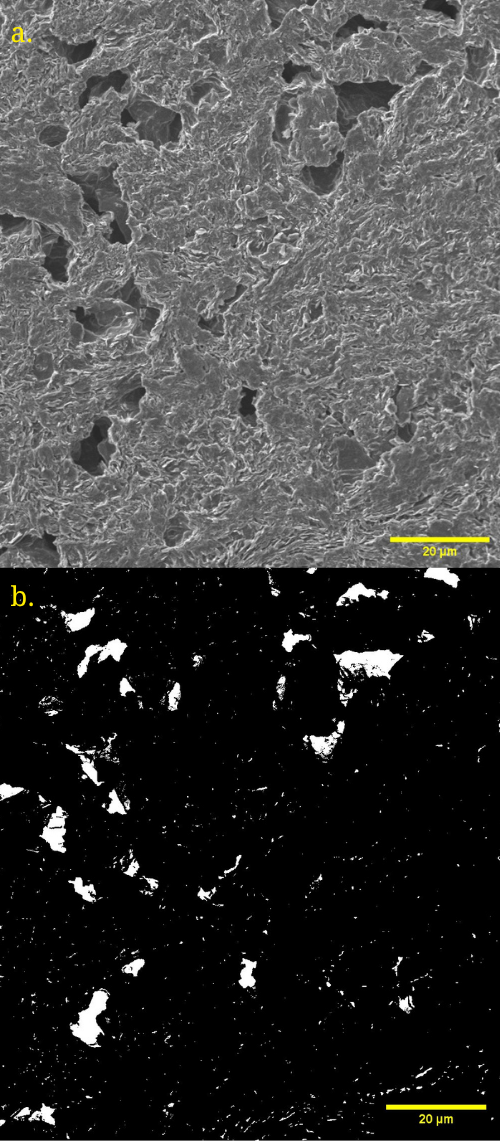
\includegraphics[width=0.45\textwidth]{./Media/intensitythresholdexampleig430fdual.png}
    \caption{DRAFT: IG430F raw (a) and following intensiy thresholding (b)}
    \label{fig:dualintensitythreshig430f}
\end{figure}

	\subsubsection{Pore Diameter Thresholding}
    
  Pore size thresholds were imposed in this work, as in previous studies
  \citep{Taylor2016, Huang2019, Kane2011a}, to restrict the automated
  recognition of pores to a range (i.e., only counting pores > 12.5 µm$^2$)
  where classification is deemed reliable. This approach is inherently
  limited by the practical difficulty of objectively determining whether any
  given pore classification is correct.
      
  As  in (Table ~\ref{tab:thresholdsandvariationsIG430F}), significant changes
  in the total pore count result from minor alterations in the threshold.
  However, the total area of pores exhibits far less variation as a function of
  pore diameter threshold (Table ~\ref{tab:thresholdsandvariationsIG430F}). When
  combined with individual analyses of the resulting PSDs and sensitivity
  analysis at each threshold as per (Figure ~\ref{fig:improvedporediademo}), a
  pore area threshold of 1 µm\(^2\) (diameter = 1.12 µm) was selected as a compromise
  between type I and II errors.\todo{Does it make sense to say this about I and II errors}

   Crucially, setting such a threshold does not imply that no pores exist below
   this limit. Rather, it acknowledges that the confidence in classifying pores
   below the threshold is too low for reliable use. In this work, the
   limitations of any single technique are compensated by the strengths of
   others. during modelling, an interval is selected over which the channel
   porosity determined from SEM imaging can reliably constrain the outputs of
   the inverse modelling process. Thus, no type II errors are introduced in the
   final model due to pore size thresholding, thanks to the combined use of
   alternative techniques and the ability to specify an interval within
   PoreXpert v.3.

   \todo{This part really requires Peter's insight as to the actual functioning of the program}
   \todo{This is not the key issue. The real thing is the accuracy of the pore
   size distribution generated by SEM. For example, the modelling would I think
   be distorted completely by saying that 3\% of the sample surface is made up
   of pores of 1.12-25 µm diameter, when that number may actually represent all
   pores above 1.12 µm, and it is just fragmenting the pores. Being unsure about
   the exact diameter range of pores covered by SEM must surely be making the 
   modelling less accurate, and the pore size distribution more skewed.}

   \begin{table}
  \centering
  \caption{Effect of different pore area thresholds on a subsection of IG-430F, showing the resulting pore count, total area, average pore size, and percentage area.}
  \label{tab:thresholdsandvariationsIG430F}
  \resizebox{\columnwidth}{!}{%
    \begin{tabular}{l c c c c c c}
      \hline
      \textbf{Area Threshold} ($\mu$m$^2$) & 0 & 0.5 & 1 & 2 & 4 & 8 \\
      \hline
      Count & 254261 & 11375 & 6 & 4085 & 2812 & 1881 \\
      Total Area (µm²) & 71219 & 56722 & 53361 & 50063.63 & 46518 & 41161\\
      Average Size (µm²) & 0.28 & 4.987 & 8.229 & 12.255 & 16.543 & 21.883 \\
      \% Area & 4.786 & 3.812 & 3.586 & 3.364 & 3.126 & 2.766 \\
      \hline
    \end{tabular}%
  }
\end{table}

\begin{figure}[!htbp]
    \centering
    \includegraphics[width=0.35\textwidth]{./Media/ImprovedPoreDiaDemo.png}
    \caption{Effect of minimum area threshold on pore identification in subsample of IG-110 Sample B. Highlighted circles denote features which surpassed the previous threshold(s) only, indicated by colour. Thresholds applied (a–f, left-to-right, top-to-bottom): None, 0.5 µm\(^2\), 1 µm\(^2\), 2 µm\(^2\), 4 µm\(^2\), and 8 µm\(^2\).}
    \label{fig:improvedporediademo}
\end{figure}

\subsubsection{Channel Porosity Analysis and Calculation}
Channel porosity was calculated using the “Analyse Particles” function in
ImageJ. This function scans the micrograph pixel by pixel, identifying pixels
suprassing the intensity threshold, and groups them into connected regions via a
flood-fill algorithm. Connectivity is defined based on the 8-connected (Moore
neighbourhood) criterion, whereby a pixel at $(x,y)$ is considered connected to
its eight immediate neighbours:
\todo{I say channel porosity here, but this needs to be made consistent everywhere}

\begin{multline*}
(x-1,y-1),\; (x-1,y),\; (x-1,y+1),\; (x,y-1),\\[4pt]
(x,y+1),\; (x+1,y-1),\; (x+1,y),\; (x+1,y+1)
\end{multline*}

Any two pixels that exceed the intensity threshold and are either directly
adjacent or diagonally connected are classified as belonging to the same region
(pore). The function then computes the area of each pore by converting the pixel
count into physical area (i.e., 10 pixels per micrometre). Regions that do not
meet the area threshold are omitted. The final results are a pore size
distribution (PSD) and the channel porosity (\%).

The result of intensity thresholding followed by pore diameter thresholding at
1.12 m diameter is exemplified, demonstrating a high degree of accuracy as
evaluated by the operator, especially given the particular focus at this stage
in excluding Type I rather Type II errors (Figure ~\ref{fig:C1-ig430f fused
cropped 8 bit one color threshed subsample 2um areathresh})

\begin{figure}[!htbp]
    \centering
    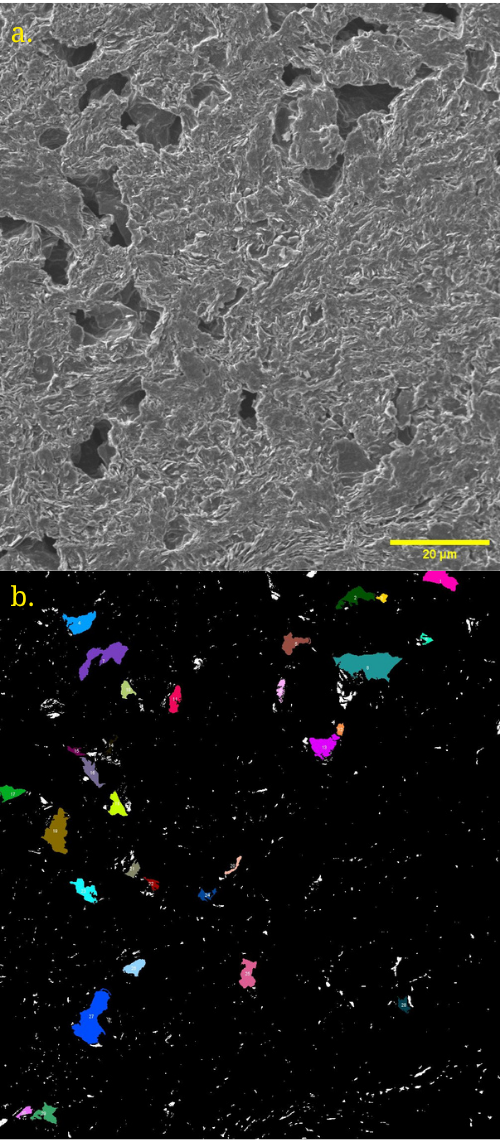
\includegraphics[width=0.45\textwidth]{./Media/C1-ig430f fused cropped 8 bit one color threshed subsample 2um areathresh}
    \caption{Draft: IG-43F subsample a. Raw and b. After intensity and pore diameter thresholding}
    \label{fig:C1-ig430f fused cropped 8 bit one color threshed subsample 2um areathresh}
\end{figure}

\subsection{Helium (He) Pycnometry}

Helium pycnometry measures the volume of solids, from which density can be
derived for a known mass, via gas displacement, applying Boyle's Law for
multiple states (Eq. \ref{eq:boylestates}). 

\begin{equation} \label{eq:boylestates}
  \mathrm{P}_{1}\,\mathrm{V}_{1} \;=\; \mathrm{P}_{2}\,\mathrm{V}_{2}.
\end{equation}

The dataset containing Skeletal density measurements, and calculations of Closed
Pore Volume (CPV), Open Pore Volume (OPV), and Specific Pore Volume (SPV)
generated by Jones et al. \citep{Jones2018} was used. This dataset represents
measurements performed on IG-110 and IG-430 sampled from the same block as those
samples which underwent SEM imaging in this work.

A Pycnomatic ATC pycnometer (Thermo Fisher Scientific, Italy) was used to
generate this dataset. Measurements were performed at a temperature of 20.00 ±
0.01\textdegree{}C,  in ten replicates per sample, calculating the arithmetic
mean. 

Solid phase volume $V_{\mathrm{SOLID}}$ was calculated assuming a theoretical
density of 2.26 g cm$^{-3}$ for an idealised graphite crystal. 

\subsection{Mercury (Hg) Intrusion Porosimetry}
Mercury intrusion porosimetry operates on the fundamental principle that the
pressure at which a non-wetting fluid intrudes a given pore is inversely
proportional to the diameter of that pore (i.e., the larger the pore, the easier
it is for the non-wetting fluid to enter it). The exact physical relationship
between diameter and applied pressure is governed by the Laplace Equation (Eq.
~\ref{eq:washburn})
	
	\begin{equation} \label{eq:washburn}
		d = \frac{-4\gamma \cos \theta}{P}
	\end{equation}

		The pore diameter \(d\) is calculated using the equation:
	\begin{itemize}
		\item $d$ (m): Pore diameter
		\item $\gamma$ (N/m): Surface tension of the fluid
		\item $\theta$ (degrees): Contact angle of the fluid with the surface
		\item $P$ (Pa): Pressure
	\end{itemize}

Values of 140$^{\circ}$ and 130$^{\circ}$ were used for advancing and receding
contact angles respectively, while a value of 0.480 N m$^{-1}$ was assumed for the
surface tension of mercury \citep{VANBRAKEL19811}.  

In this work, the dataset generated by Jones et al. \citep{Jones2018} was used,
representing measurements performed on IG-110 and IG-430 sampled from the same
block as those samples which underwent SEM imaging in this work. in this work.

\subsection{Nitrogen (N$_2$) Adsorption}
Low-pressure gas adsorption isotherms were obtained using a BELSORP-max
volumetric gas adsorption instrument (MicrotracBEL, Japan). 

The dataset generated by Jones \textit{et al}. \citep{Jones2018} was used in
this work, again representing measurements performed on IG-110 and IG-430
sampled from the same block as those samples which underwent SEM imaging in this
work.

\section{Modelling}

PoreXpert is a quasi-Bayesian model which proceeds inversely from effect (the
percolation) to cause (the void network). The software constructs an 8
dimensional parameter space,  composed of 5 numerical parameters which represent
the physical characteristics of the pore network, and 3 constraining Boolean
parameters, for example, to avoid structures where features overlap each other.
A Boltzmann-annealed amoeboid simplex searches over this parameter space to find
the set of parameters that produces a percolation curve minimally different from
the intrusion curve derived from Hg porosimetry and N$_2$/Kr adsorption. The
intrusion curve is formed of experimental output from both methods as mercury
porosimetery cannot reach sufficient pressure to probe the smallest
voids of interest, and therefore, the percolation characteristic is extended to
smaller void sizes by Grand-Canonical Monte-Carlo interpretation of N$_2$
adsorption.  The final result is a simulated pore network with the correct
porosity and percolation properties, on which many simulations, such as
pore-fluid permeability and tortuousity, and sample ageing under radiation, can
be performed (Figure \ref{fig:PX3dnetwork} \citep{MatthewsPoreXpert2025}).


\todo{roughly no more than 5 mentions of PX, call it inverse modelling package everywhere else. }
    During modelling, the approximation type that best reflects the depth of
    imaging into the porous structure is selected (Figure
    \ref{fig:pxapproxtypes}, \citep{MatthewsPoreXpert2025}). Approximation Type
    1 \textit{Surface connected throats only} is likely the optimal
    approximation for the channel porosity dataset constructed in this work, as
    a consequence of the stringent intensity threshold applied. However, due to
    stability challenges in this early compilation, approximation Type 2
    \textit{Surface connected throats and the visible volumes of connected
    pores} was applied instead (Figure ~\ref{fig:pxapproxtypes}). \todo{Without
    being able to run it, you could not verify, so I think it would be better to
    just specify the approximation type.}

   \todo{make it myself, make it clearer and nicer}
    \begin{figure}
	    \centering
	    \includegraphics[width=0.45\textwidth]{./Media/bradpxapproximationtypesv2.png}
	    \caption{Approximation types 1-4, white is the porosity which is visible
       to the SEM and black is the bulk of the sample. a. Surface connected
       throats only b. surface connected throats and the visible volumes of
       connected pores c. surface connected throats, the visible volumes of
       connected pores and any throats below them d. All vertically aligned
       features in the top layer, connected and unconnected to the surface.  }
	    \label{fig:pxapproxtypes}
	\end{figure}

  Channel porosity data were entered into the PoreXpert v.3 interface including
  a minimum and maximum pore diameter as per (Figure ~\ref{fig:Final Workflow}),
  the model was able to adjust the extent of the PSD which the channel porosity
  estimates, optimising effectively to a minimal distance distance of 1.91\%
  deviation from the experimental curve

  (Figure ~\ref{fig:PXfittinggraph})
    \begin{figure}
        \centering
        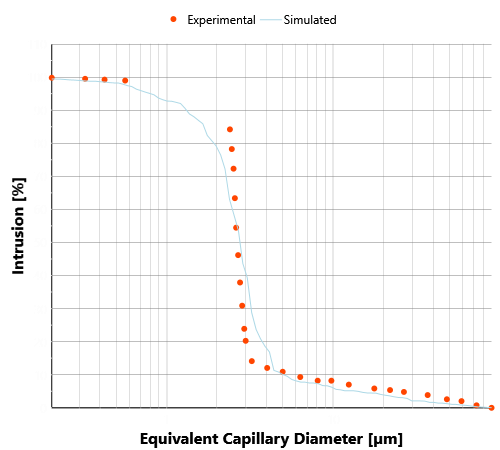
\includegraphics[width=0.45\textwidth]{./Media/Fit to percolation curve.png}
        \caption{Fitting simulated intrusion curve to experimental curve  as per (Figure ~\ref{fig:modelling
        pipeline}). Orange dots denote experimental datapoints, the blue line is
        the simulated percolation curve resulting from a pore network of
        5 numerical parameters.}
        \label{fig:PXfittinggraph}
    \end{figure}


      \begin{figure}
        \centering
        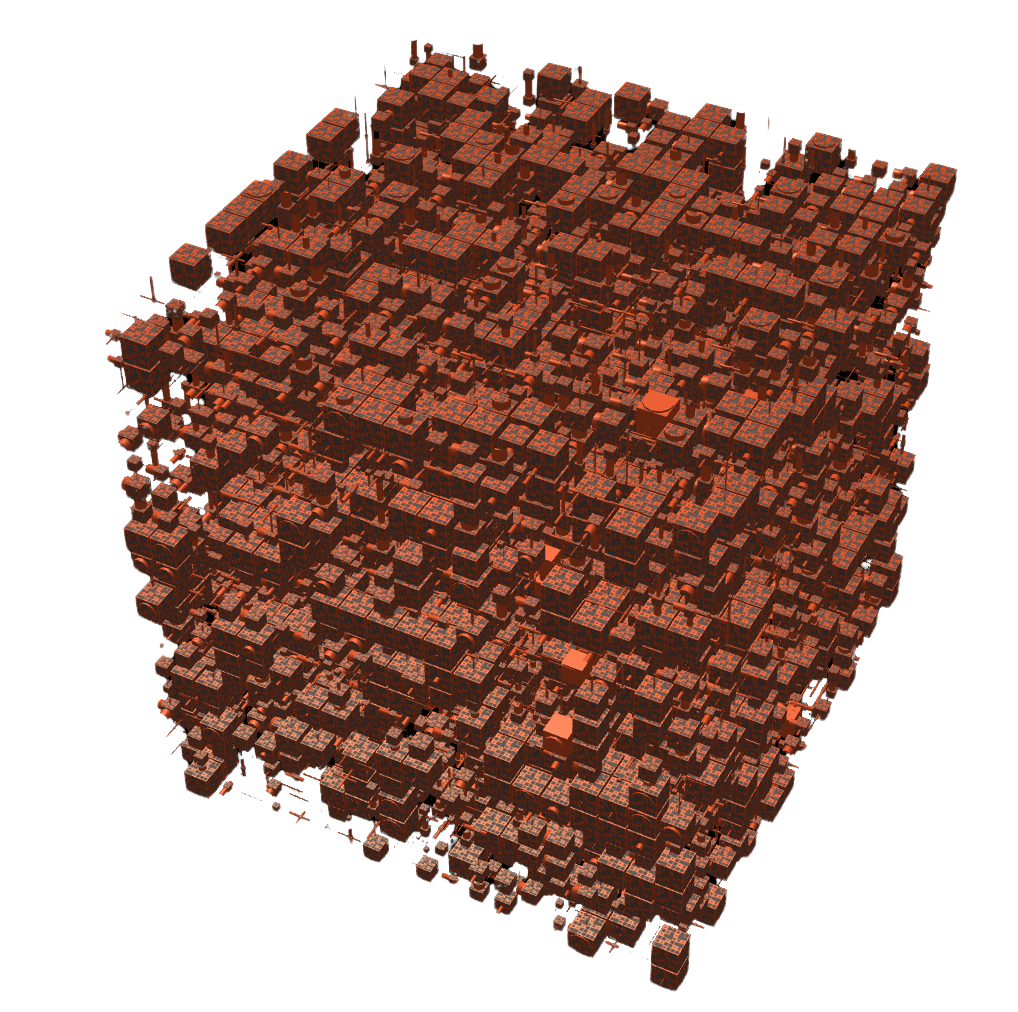
\includegraphics[width=0.45\textwidth]{./Media/unit cell no bg.png}
        \caption{Visualisation of the pore network resulting from the
        integration of channel porosity and experimental data by the workflows
        above. 1.91\% distance between simulated and experimental curves,
        following the application of Approximation Type 2 (Figure
        ~\ref{fig:pxapproxtypes}). Channel Porosity estimation was averaged over
        the top 9 layers of a unit cell 20x20x20. The result of one generation
        of stochastic number generation. Run in Direct Mode as Batch mode
        remained unstable in this early compilation}
        \label{fig:PX3dnetwork}
    \end{figure}

    Initial outputs of PoreXpert modelling are congruent with manuafcturer data
    with manufacturer datasets, as exemplified for IG-110 Sample B.
    Crucially, the linear trend line shows only a weak correlation between open
    porosity estimate and distance between simulated and experimental
    percolation characteristic (r\(^2\) = 0.32) (Figure
    \ref{fig:validationgraph}). Thus, taking the average over all stochastic
    generations is a valid measure of this method's estimate of
    open porosity. 

\begin{figure}
    \centering
    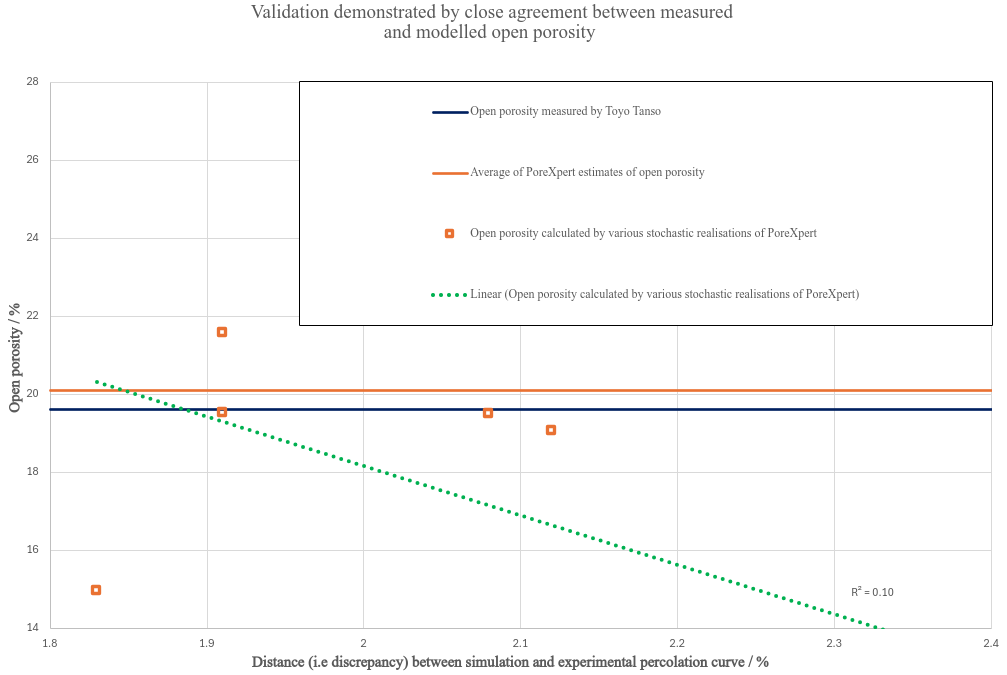
\includegraphics[width=0.45\textwidth]{./Media/ValidationGraph.png}
    \caption{DRAFT: Needs to be reformatted for publicatiom, if we choose to keep it.Validation of modelled open porosity by comparison of modelled open porosities generated by PoreXpert with manufacturer data for IG-110, which estimates a 19.62\% open porosity \cite{Jones2018}}
    \label{fig:validationgraph}
\end{figure}

  Initial modelling generated plausible data…

\section{Results}

\begin{table}
  \centering
  \caption{Pore Size Distribution (PSD) and summary characteristics for IG-110 and IG-430 samples, tabulating number of pores, total pore area, and channel porosity.}
  \label{tab:PSDtable}
  \resizebox{\columnwidth}{!}{%
    \begin{tabular}{c c c c}
      \hline
      Sample & n / pores & Total Area / $\mu$m$^2$ & Channel Porosity / \% \\
      \hline
      IG110 B & 8,684  & 41,091 & 3.14 \\
      IG110 C & 7,075  & 49,755 & 3.27 \\
      IG110 F & 8,296  & 50,735 & 3.38 \\
      IG430 B & 6,848  & 32,983 & 2.30 \\
      IG430 C & 13,026 & 49,534 & 2.94 \\
      IG430 F & 6,819  & 56,794 & 3.66 \\
      \hline
    \end{tabular}%
  }
\end{table}

The completed workflow of SEM imaging and computational composite analysis
yielded estimates of channel porosity for both graphite grades (Table
~\ref{tab:PSDtable}). IG-110 samples exhibited channel porosity values ranging
from 3.14-3.38\%, while IG-430 samples showed greater variability, ranging from
2.30-3.66\%

\begin{figure}
    \centering
    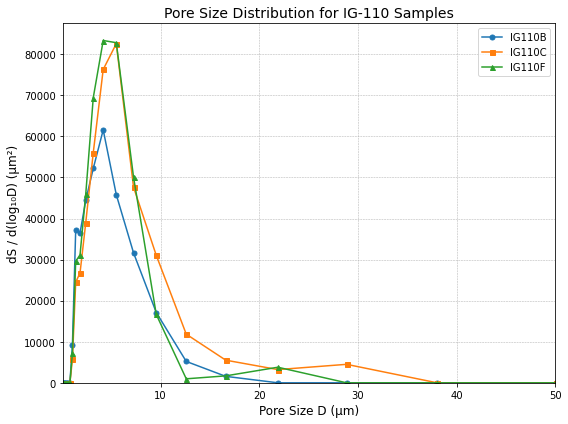
\includegraphics[width=0.45\textwidth]{./Media/IG110 ds LogD .png}
    \caption{DRAFT: I want to recheck my code on these distributions}
    \label{fig:IG110LogPSDs}
\end{figure}

\begin{figure}
    \centering
    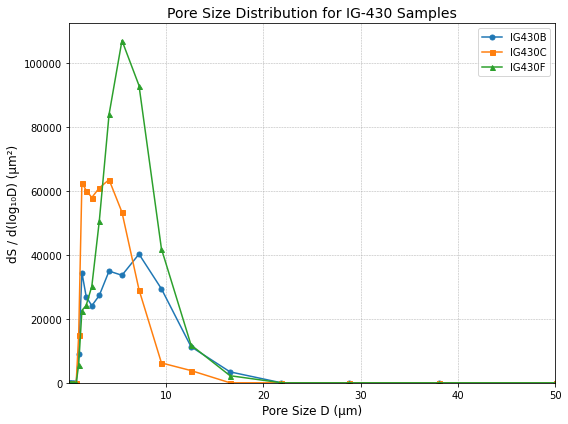
\includegraphics[width=0.45\textwidth]{./Media/IG430 ds LogD .png}
    \caption{DRAFT: I want to recheck my code on these distributions}
    \label{fig:IG430LogPSDs}
\end{figure}

Area contribution distribution is represented graphically for both graphite
grades (Figure ~\ref{fig:IG110LogPSDs}, ~\ref{fig:IG430LogPSDs}). The area of
each logarithmic bin (spanning 0.1-100 µm on the x-axis) was summed then divided
by the bin width in \(\log_{10}(D)\) to derive \(dS/d(\log_{10}D)\), with the
x-axis then linearised.  y-axis values represent area density in µm\(^2\) per
\(\log_{10}(D)\).

IG-110 and IG-430 both exhibit a peak in the sub-10 µm range. This is the
inverse of trends observed in previous OM-based analyses, where the majority of
the porosity is contributed by pores above this range \citep{Huang2019}.
\citep{huang2021statistical} found that porosity as by classified SEM, albeit 
with a different distribution, was 3\% for IG-110, which is highly
congruent with the 3.14-3.38\% range derived in this work.

Interpolation increases confidence in the basic functionality of this method.
Adjustment of the intensity threshold to match previous OM works (i.e., pore
contours and pore throats are no longer distinguished, via a reduction in
intensity threshold) produces highly similar channel porosity values.
Specifically, \citep{Kane2011a} estimated a channel porosity of 14.73\% for
IG-110, with \citep{Huang2019} deriving 14\% for the same grade, highly
congruent with the approximately 13-14\% figure this method derives with an
adjusted intensity threshold, but also illustrating the scale of the impact in
intensity threshold selection on the final channel porosity estimate.

\section{Discussion}

  \subsection{Channel Porosity Overestimation due to connecitivity algo}
  This algorithm is likely to yield at least a  slight overestimation of the
channel porosity. This is because such an inclusive definition means that two or
more pores, connected by a narrow neck or even simply with adjacent pixels,
would be classified as a single pore. Notably, this would not change the final
channel porosity (\%), at least in isolation, but would result in a rightward
shift in the PSD. Skeleton segmentation is for fine-grade nuclear graphite
likely to be a more accurate approach than a simple connectivity algorithm as
used here would be a key improvement if implemented
\cite{ARREGUIMENA2022112047}

\subsection{Pore Fragmentation and Implications for Modelling}
The application of a maximum pore diameter is a key part of the modelling as
  initial modelling where this was not implemented failed to yield reliable
  results. It is believed that this is due to the impossiblity of the model
  fitting an plausible network on the premise that pores from 1.12 µm diameter
  upwards represent only 3 \% of the sample surface. Imposing an upper threshold
  as the simple max of the pore diameters identified by SEM is an uncomplicated
  initial solution which has more logical implications (i.e., to state that
  between 1.12 and 20um diameter, 3\% of the sample surface is represented by
  porosity). This threshold varied between 13-26 µm in this work, which should
  cover the vast majority of the porosity, particularly given the pore fragmentation
  issue described below.

  Specifically, the use of a simple Moore neighbourhood connectivity, when
  combined with the fact that Erosion and Dilation binary operations were not
  applied, means that pores which the operator identifies as a single pore are
  in more than one case instead defined as two or more pores. Not only this but
  these split pores may not then surpass the pore diameter threshold of 1.12um.
  (e.g., a pore of 10um diameter might be split into 2 pores, 1 of 9um diameter
  and another of 1um diameter, which would be discarded due to the pore diameter
  threshold, reducing the channel porosity \% and shifting rightward the pore
  size distribution).

  The end result is that it is difficult to describe the pore size distribution
  derived from SEM as it currently stands, as completely impenetrable.
  Crucially, the production of reasonable results from the modelling as above
  depends on an accurate constraint of the pore diameter interval (i.e., the
  channel porosity figure of 3\% refers only to porosity between 1.12 and 25um
  diameter) and so not only the SEM-derived pore size distribution but the PX
  modelling which uses it, has at least some reduction in reliability due to the
  pore fragmentation issue. However, this is likely a soluble problem, as follows.

  \subsection{Proposed Future Workflow}

  -Just my idea of an improved workflow:
  1. Resin Impregnation
  2. SEM (see if we can go to 2kV)
  3. Otsu Thresholding (We have clear bimodality thanks to Resin impregnation)
  4. Skeleton segmentation (Avizo software needed?)
  5. Apply improved pore diameter thresholds, or maybe do not do any at all as no longer needed? At least lowered.
  6. Modelling

\section{Supplementary Information}

One advantage of this method is the avoidance of error propagation by
consecutive registration steps, as simply placing micrograph A relative to
micrograph B, and then micrograph B relative to micrograph C, would result in
accumulation of errors. This method builds a graph whose nodes are the
micrographs, and edges are the measured pairwise shifts between the micrographs.
It then finds the set of micrograph positions that minimise the total squared
registration error across the entire graph, a form of globally optimised
registration \citep{Preibisch2009}.

This stitching method also allows sub-pixel accuracy, which is crucial for
accurate pore measurement. For any two micrographs \(A\) and \(B\), which are
shifted relative to each other (i.e., micrograph \(B\) is shifted two pixels up
and 10 pixels left of micrograph \(A\)) then their Fourier transforms would
have the same magnitude but different phases. A normalized cross-power spectrum
isolates the phase difference, and the Inverse Fourier transform
yields a correlation map with peaks indicating possible translations between the
micrographs. The complexity of real images and the periodicity of the Fourier
transform means that the correlation map is not a single peak, but rather a set
of peaks, each representing a possible translation. This method therefore
selects the \(n\) highest local maxima and finds the peak with the best
correlation, which it defines as the true translation between the two
micrographs \citep{Preibisch2009}. Finally, sub-pixel accuracy in that shift is
achieved by applying a parabolic interpolation around the selected peak to
refine the translation estimate.

Additionally, a non-linear intensity blending function eliminates the visible
seams between micrographs, which can occur even when the micrographs are
perfectly aligned due to shading variations. This blending assigns a weight to
each pixel in a tile, working as a function of the distance from the tile edge,
with a tunable parameter controlling this weighting function. In
non-overlapping regions, the centre of the micrograph, the weight is essentially
1, so the original pixel value is preserved exactly. In overlapping regions,
intensities are a convex combination of the original values. Crucially, because
the weights sum to 1 everywhere, blended intensity is simply a weighted average
of the original intensities. Thus, the final composite micrograph is still a
valid representation of the original micrographs, but the seams have been
removed.  \citep{Preibisch2009} Testing indicated that adjustment of the
blending parameter \(a\) had no discernable impact on the final composite
micrograph, and therefore no impact on the final porosity values. Inversely, the
removal of the visible seams between micrographs did increase confidence that in
the following steps, the subsample used to determine the intensity threshold was
representative of the full composite micrograph.
\clearpage

\bibliography{bibliography}
\end{document}